\chapter{Introduction}

\tab Software systems are continuously in change. As long as the software system is used the changing process is never finished. Changes can be triggered by new features, defects, new technologies, system refactoring for maintainability.\\ Software maintenance can be made during the development process by maintaining the already implemented features, while developing new ones or at the end of the development process when the system is no longer open to new features requested by the client and the maintenance is only made for the existing ones.\\

\tab A system is stable when a change in one component of the system does not affect the other components .This rule applies recursively also inside the components.
In this paper we intend to understand better the intersection between structural dependencies and logical dependencies and their impact over the system stability (Figure \ref{fig:fig2}). We also would like to study multiple ways of building and filtering logical dependencies and how this can affect the final result of the analysis.

\begin{figure}[h]
\centering
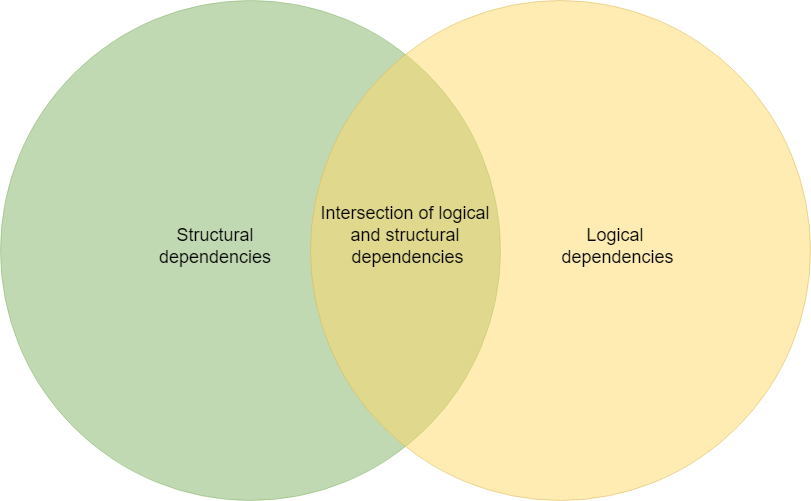
\includegraphics[scale=0.4]{fig2.png}
\caption{Venn Diagram showing the intersection between structural and logical dependencies }
\label{fig:fig2}
\end{figure}